\documentclass[lang=cn,a4paper,newtx,bibend=bibtex]{elegantpaper}
\usepackage{env}
\title{Problems of Chapter 11}
\author{张志心 \ 计科2106}
\date{\zhdate{2024/06/11}}
\pgfplotsset{compat=1.17}
\addbibresource[location=local]{reference.bib}
\begin{document}
\maketitle

\begin{prob}[Exercise 11.11]
  Show that the matrix form of the Crank-Nicolson method
  for solving the heat equation (11.3) with Dirichlet condition is
  \begin{equation*}
    (I-\frac k2A) \UB^{n+1} = (I+\frac k2A) \UB^n + \bB^n,
  \end{equation*}
  where
  \begin{equation*}
    \bB^n = \frac r2
    \MAT{
      g_0(t_n) + g_0(t_{n+1}) \\
      0 \\
      \vdots \\
      0 \\
      g_1(t_n) + g_1(t_{n+1}) \\
    }
  \end{equation*}
\end{prob}

\begin{solution}
  根据定义 11.10 得
  \begin{equation*}
    \dfrac{U_i^{n+1} - U_i^n}k = \frac 12\left(f(U_i^n, t_n) + f(U_i^{n+1}, t_{n+1})\right)
  \end{equation*}
  即
  \begin{equation*}
    U_i^{n+1} - \frac k2 f(U_i^{n+1}, t_{n+1}) = U_i^n + \frac k2 f(U_i^n, t_n)
  \end{equation*}
  代入半离散系统 $\UB' = A\UB + \gB$ 得
  \begin{equation*}
    \UB^{n+1} - \frac k2 (A\UB^{n+1} + \gB^{n+1}) = \UB^n + \frac k2 (A\UB^n + \gB^n).
  \end{equation*}
  整理得
  \begin{equation*}
    (I - \frac k2 A)\UB^{n+1} = (I + \frac k2 A)\UB^n + \frac k2(\gB^n + \gB^{n+1}).
  \end{equation*}
  因为
  \begin{equation*}
    \frac k2(\gB^n + \gB^{n+1}) = \frac {k\nu}{2h^2}
    \MAT{ g_0(t_n) + g_0(t_{n+1}) \\ 0 \\ \vdots \\ 0 \\ g_1(t_n) + g_1(t_{n+1})}
    = \bB^n,
  \end{equation*}
  所以待证式成立。
\end{solution}

\begin{prob}[Exercise 11.26]
  Prove Lemma 11.25 via the stability function of one-step methods.
\end{prob}

\begin{solution}
  根据单步法的稳定性函数定义,我们将 $\theta-$method 的半离散格式
  \begin{equation*}
    \UB^{n+1} = \UB^n + k(\theta f(U^{n+1}) + (1-\theta)f(U^n))
  \end{equation*}
  应用于方程 $u' = \lambda u$ 得
  \begin{equation*}
    U^{n+1} = U^n + k(\theta\lambda U^{n+1} + (1-\theta)\lambda U^n).
  \end{equation*}
  整理得
  \begin{equation*}
    U^{n+1} = \dfrac{1+k(1-\theta)\lambda}{1-k\theta\lambda}U^n.
  \end{equation*}
  代入 $z=k\lambda$ 得稳定性函数为
  \begin{equation*}
    R(z) = \dfrac{1+(1-\theta)z}{1-\theta z}.
  \end{equation*}
  要使上述格式稳定,我们需要对一切特征值 $\lambda$ 均有
  \begin{equation*}
    |R(k\lambda)|\leq 1+O(k).
  \end{equation*}
  注意到 $-\dfrac{4\nu}{h^2}\leq \lambda < 0$,
  而当 $\theta\in [\frac 12,1]$ 时,$|R(z)|\leq 1$ 对一切 $z\leq 0$ 恒成立。
  故此时 $\theta-$method 无条件稳定。
  当 $\theta\in [0,\frac 12)$ 时,解不等式可得
  \begin{equation*}
    z\geq \dfrac{-2}{1-2\theta}.
  \end{equation*}
  故 $k$ 需要满足 $\dfrac{-2}{1-2\theta}\leq -\dfrac{4\nu}{h^2}k$。
  即 $k\leq \dfrac{h^2}{2(1-2\theta)\nu}$。
\end{solution}

\begin{prob}[Exercise 11.41]
  Show that any grid function in $L^1(h\ZBB)$ can be recovered by a Fourier transform
  followed by an inverse Fourier transform.
\end{prob}

\begin{solution}
  设 $\UB\in L^1(h\ZBB), U(hj) = U_j$。则由 Lemma 11.39 得
  \begin{equation*}
    \begin{aligned}
      & (\FM^{-1}\FM)(U)_n & \\
      = & \FM^{-1}(\FM U)_n & \\
      = & \FM^{-1}(\frac 1{\sqrt{2\pi}}\sum_{m\in \ZBB}e^{-\ii mh\xi}U_mh)_n & \\
      = & \frac 1{2\pi}\int_{-\frac{\pi}h}^{\frac{\pi}h}e^{\ii nh\xi}\sum_{m\in \ZBB}e^{-\ii mh\xi}U_mh\dd\xi & \\
      = & \frac 1{2\pi}\int_{-\frac{\pi}h}^{\frac{\pi}h}\sum_{m\in \ZBB}e^{\ii(n-m)h\xi}U_mh\dd \xi & \\
      = & \frac 1{2\pi}\int_{-\frac{\pi}h}^{\frac{\pi}h}U_nh\dd\xi & \\
      = & U_n. & \\
    \end{aligned}
  \end{equation*}
\end{solution}

\begin{prob}[Exercise 11.48]
  Prove Lemma 11.25 via Von-Neumann analysis.
  What can you say after comparing this proof with that for Exercise 11.26?
\end{prob}

\begin{solution}
  对迭代式
  \begin{equation*}
    -\theta rU_{j-1}^{n+1} + (1 + 2\theta r)U_j^{n+1} - \theta rU_{j+1}^{n+1}
    = (1-\theta)rU_{j-1}^n + [1 - 2(1-\theta)r]U_j^n + (1-\theta)rU_{j+1}^n.
  \end{equation*}
  两端同时 Fourier 变换,即代入(11.48)式得
  \begin{equation*}
    \begin{aligned}
      & \frac 1{\sqrt{2\pi}}\int_{-\frac{\pi}h}^{\frac{\pi}h}\left(-\theta re^{\ii (j-1)h\xi} + (1+2\theta r)e^{\ii jh\xi} - \theta re^{\ii(j+1)h\xi}\right)\hat{U}^{n+1}(\xi)\dd \xi & \\
    = & \frac 1{\sqrt{2\pi}}\int_{-\frac{\pi}h}^{\frac{\pi}h}\left((1-\theta)re^{\ii(j-1)h\xi} + [1-2(1-\theta)r]e^{\ii jh\xi} + (1-\theta)re^{\ii(j+1)h\xi}\right)\hat{U}^n(\xi)\dd \xi. & \\
  \end{aligned}
\end{equation*}
  设 $\hat{U}^{n+1} = \hat{U}^n(\xi)g(h\xi)$,则
  \begin{equation*}
    g(h\xi) = \dfrac{(1-\theta)re^{\ii(j-1)h\xi} + [1-2(1-\theta)r]e^{\ii jh\xi} + (1-\theta)re^{\ii(j+1)h\xi}}{-\theta re^{\ii(j-1)h\xi} + (1+2\theta r)e^{\ii jh\xi} - \theta re^{\ii(j+1)h\xi}}
    = \dfrac{2(1-\theta)r\cos(h\xi) + 1-2(1-\theta)r}{-2\theta r\cos(h\xi) + 1+2\theta r}.
  \end{equation*}
  $\theta-$method 稳定需要$|g(h\xi)| \leq 1+O(k), \forall \xi\in [-\frac{\pi}h, \frac{\pi}h]$。
  当 $\theta\in [\frac 12, 1]$ 时不等式恒成立,故该方法无条件稳定。
  当 $\theta\in [0,\frac 12)$ 时,解得 $r\leq \dfrac 1{(1-2\theta)(1-\cos(h\xi))}$。
  因为 $-1\leq \cos(h\xi)\leq 1$,所以 $r\leq \dfrac 1{2(1-2\theta)}$。
  即 $k\leq \dfrac {h^2}{2(1-2\theta)\nu}$。
\end{solution}

\begin{prob}[Exercise 11.78]
  Show that the Beam-Warming method is second-order accurate both in time and in space.
\end{prob}

\begin{solution}
  我们只证明 $a\geq 0$ 时的情形,$a<0$ 同理。
  \begin{equation*}
    \begin{aligned}
      & \tau(x,t) & \\
      = & u(x_j, t_n+k) - u(x_j, t_n) - \frac {\mu}2(3u(x_j, t_n) - 4u(x_{j-1}, t_n) + u(x_{j-2}, t_n)) + \frac{\mu^2}2(u(x_j, t_n) - 2u(x_{j-1}, t_n) + u(x_j, t_n)) & \\
      = & u + ku_t + \frac {k^2}2 u_{tt} - u -\frac {\mu}2(3u - 4(u+u_x+\frac{h^2}2u_{xx}) + \\
        & (u-2hu_x+2h^2u_{xx})) + \frac{\mu^2}2(u - 2(u-hu_x+\frac{h^2}2u_{xx}) + (u-2hu_x+2h^2u_{xx})) + O(k^3+h^3) & \\
      = & ku_t + \frac{k^2}2u_{tt} + \mu hu_x + \frac{\mu^2}2u_{xx} + O(h^3+k^3) & \\
      = & -aku_x + \frac{a^2k^2}2u_{xx} + aku_x + \frac{a^2k^2}2u_{xx} + O(h^3+k^3) & \\
      = & a^2k^2u_{xx} + O(h^3+k^3) & \\
    \end{aligned}
  \end{equation*}
  因此 Beam-Warming 方法具有二阶时空精度。
\end{solution}

\begin{prob}[Exercise 11.79]
  Show that the Beam-Warming methods (11.86) and (11.87) are stable
  for $\mu\in [0,2]$ and $\mu\in [-2,0]$, respectively.
  Reproduce the plot in Figure 11.6.
\end{prob}

\begin{solution}
  只证明 $a\geq 0$ 的情形,$a<0$ 同理。
  当 $a\geq 0$ 时,$\mu = \frac{ak}{h}\geq 0$。
  Beam-Warming 方法的半离散系统为
  \begin{equation*}
    \UB'(t) = B\UB(t),
    B = -\frac{k\mu}2\MAT{
      3 & & & \dots & 1 & -4 \\
      -4 & 3 & & \dots & & 1 \\
      1 & -4 & 3 & \dots & & \\
      & \ddots & \ddots & \ddots & & \\
      & \dots & 1 & -4 & 3 & \\
      & \dots & & 1 & -4 & 3 \\
    }
    + \frac{k\mu^2}2\MAT{
      1 & & & \dots & 1 & -2 \\
      -2 & 1 & & \dots & & 1 \\
      1 & -2 & 1 & \dots & & \\
      & \ddots & \ddots & \ddots & & \\
      & \dots & 1 & -2 & 1 & \\
      & \dots & & 1 & -2 & 1 \\
    }
  \end{equation*}
  因为
  \begin{equation*}
    B\wB^p = \left(-\dfrac{k\mu}{2}(3-4e^{-2\pi\ii ph}+e^{-4\pi\ii ph}) + \dfrac{k\mu^2}{2}(1-2e^{-2\pi\ii ph}+e^{-4\pi\ii ph})\right)\wB^p.
  \end{equation*}
  所以 $z_p = k\lambda_p = e^{-2\pi\ii ph}\left[(\mu^2-2\mu)(cos(2\pi ph)-1) - i\mu\sin(2\pi ph)\right]$。
  当 $\mu\in [0,2]$ 时,
  \begin{equation*}
    \begin{aligned}
      1+z_p = & e^{-2\pi\ii ph}[(\mu^2-2\mu)(\cos(2\pi ph)-1) - \ii\mu\sin(2\pi ph) + e^{2\pi\ii ph}] & \\
      = & e^{-2\pi\ii ph}[(\mu-1)^2\cos(2\pi ph) + \mu(2-\mu) - \ii(\mu-1)\sin(2\pi ph)] & \\
      = & e^{-2\pi\ii ph}[\eta^2\cos(2\pi ph) + 1-\eta^2 - i\eta\sin(2\pi ph)]. & \\
    \end{aligned}
  \end{equation*}
  这里 $\eta = \mu-1\in [-1,1]$。
  取模长平方,得
  \begin{equation*}
    \begin{aligned}
      |1+z_p|^2 = & (\eta^2\cos(2\pi ph) + 1-\eta^2)^2 + (\eta\sin(2\pi ph))^2 & \\
      = & \eta^4\cos^2(2\pi ph) + 2\eta^2(1-\eta)\cos(2\pi ph) + (1-\eta^2)^2 + \eta^2(1-\cos^2(2\pi ph)) & \\
      = & \eta^2(\eta^2-1)(\cos(2\pi ph)-1)^2 \leq 1. & \\
    \end{aligned}
  \end{equation*}
  所以 Warm-Beamer 算法在 $\mu\in [0,2]$ 时绝对稳定。
  \begin{lstlisting}
mu_values = [0.8, 1.6, 2.0, 2.4];
m = 64;
theta = linspace(0, 2*pi, 1000);
C = exp(1i * theta) - 1;

figure;

for k = 1:length(mu_values)
    mu = mu_values(k);
    eigens = zeros(1, m+1);
    for I = 0:m
        eigens(I+1) = -mu/2 * (3 - 4*exp(-2i*pi*I/m) + exp(-4i*pi*I/m)) + mu^2/2 * (1 - 2*exp(-2i*pi*I/m) + exp(-4i*pi*I/m));
    end
    subplot(2, 2, k);
    scatter(real(eigens), imag(eigens), 'r');
    hold on;
    plot(real(C), imag(C));
    hold off;
    grid on;
    xlabel('Real Part');
    ylabel('Imaginary Part');
    title(['Eigenvalues for \mu = ', num2str(mu)]);
end
  \end{lstlisting}
  \begin{figure}[H]
    \centering
    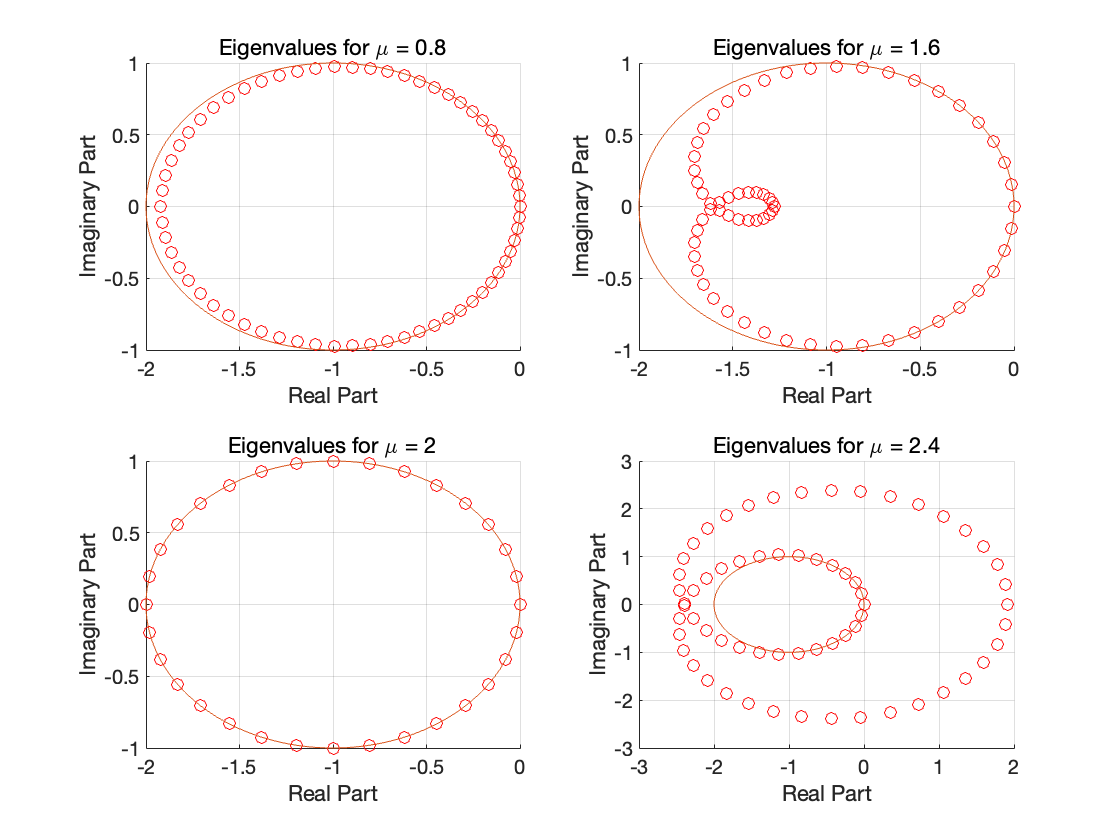
\includegraphics[width=0.7\textwidth]{1.png}
  \end{figure}
\end{solution}

\begin{prob}[Exercise 11.82]
  Plot the numerical domains of dependence of the grid point $(x_j,t_3)$
  for the upwind method with $a<0$ and $\mu=0,1,2$.
\end{prob}

\begin{solution}
  ~~\\
  \begin{figure}[h]
    \begin{minipage}{0.32\linewidth}
      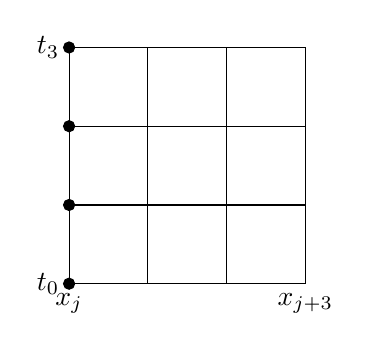
\begin{tikzpicture}
        \draw (0,0) node[below] {$x_j$} node[left] {$t_0$};
        \draw (0,0)--(0,3);
        \draw (1,0)--(1,3);
        \draw (2,0)--(2,3);
        \draw (3,0) node[below] {$x_{j+3}$};
        \draw (3,0)--(3,3);
        \draw (0,0)--(3,0);
        \draw (0,1)--(3,1);
        \draw (0,2)--(3,2);
        \draw (0,3)--(3,3);
        \draw (0,3) node[left] {$t_3$};
        \filldraw [black] (0,0) circle (2pt);
        \filldraw [black] (0,1) circle (2pt);
        \filldraw [black] (0,2) circle (2pt);
        \filldraw [black] (0,3) circle (2pt);
      \end{tikzpicture}
      \centerline{$\mu=0$}
    \end{minipage}
    \begin{minipage}{0.32\linewidth}
      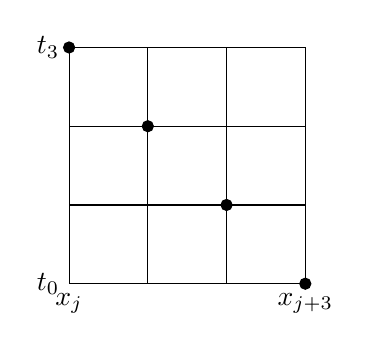
\begin{tikzpicture}
        \draw (0,0) node[below] {$x_j$} node[left] {$t_0$};
        \draw (0,0)--(0,3);
        \draw (1,0)--(1,3);
        \draw (2,0)--(2,3);
        \draw (3,0) node[below] {$x_{j+3}$};
        \draw (3,0)--(3,3);
        \draw (0,0)--(3,0);
        \draw (0,1)--(3,1);
        \draw (0,2)--(3,2);
        \draw (0,3)--(3,3);
        \draw (0,3) node[left] {$t_3$};
        \filldraw [black] (3,0) circle (2pt);
        \filldraw [black] (2,1) circle (2pt);
        \filldraw [black] (1,2) circle (2pt);
        \filldraw [black] (0,3) circle (2pt);
      \end{tikzpicture}
      \centerline{$\mu=-1$}
    \end{minipage}
    \begin{minipage}{0.32\linewidth}
      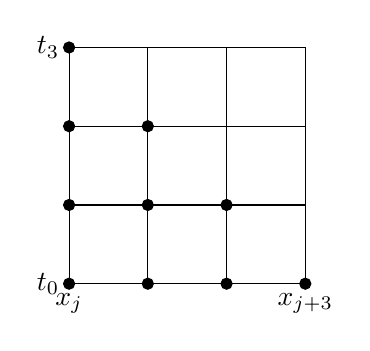
\begin{tikzpicture}
        \draw (0,0) node[below] {$x_j$} node[left] {$t_0$};
        \draw (0,0)--(0,3);
        \draw (1,0)--(1,3);
        \draw (2,0)--(2,3);
        \draw (3,0) node[below] {$x_{j+3}$};
        \draw (3,0)--(3,3);
        \draw (0,0)--(3,0);
        \draw (0,1)--(3,1);
        \draw (0,2)--(3,2);
        \draw (0,3)--(3,3);
        \draw (0,3) node[left] {$t_3$};
        \filldraw [black] (3,0) circle (2pt);
        \filldraw [black] (2,0) circle (2pt);
        \filldraw [black] (2,1) circle (2pt);
        \filldraw [black] (1,0) circle (2pt);
        \filldraw [black] (1,1) circle (2pt);
        \filldraw [black] (1,2) circle (2pt);
        \filldraw [black] (0,0) circle (2pt);
        \filldraw [black] (0,1) circle (2pt);
        \filldraw [black] (0,2) circle (2pt);
        \filldraw [black] (0,3) circle (2pt);
      \end{tikzpicture}
      \centerline{$\mu=-2$}
    \end{minipage}
  \end{figure}
\end{solution}

\begin{prob}[Exercise 11.83]
  Plot the numerical domains of dependence of the grid point $(x_j,t_3)$
  for the Lax-Wendroff method with $\mu=+1,-1$.
\end{prob}

\begin{solution}
  ~~\\
  \begin{figure}[h]
    \begin{minipage}{0.5\linewidth}
      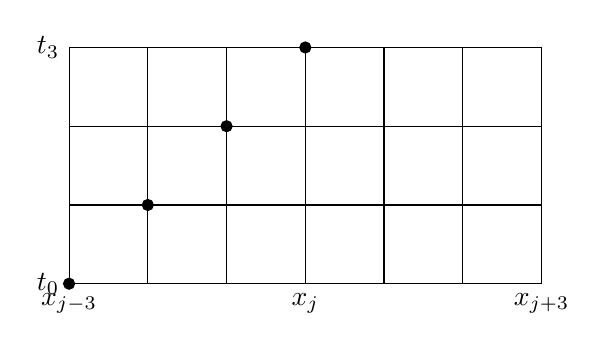
\begin{tikzpicture}
        \draw (0,0) node[below] {$x_{j-3}$} node[left] {$t_0$};
        \draw (0,0)--(0,3);
        \draw (1,0)--(1,3);
        \draw (2,0)--(2,3);
        \draw (3,0)--(3,3);
        \draw (3,0) node[below] {$x_j$};
        \draw (4,0)--(4,3);
        \draw (5,0)--(5,3);
        \draw (6,0)--(6,3);
        \draw (6,0) node[below] {$x_{j+3}$};
        \draw (0,0)--(6,0);
        \draw (0,1)--(6,1);
        \draw (0,2)--(6,2);
        \draw (0,3)--(6,3);
        \draw (0,3) node[left] {$t_3$};
        \filldraw [black] (0,0) circle (2pt);
        \filldraw [black] (1,1) circle (2pt);
        \filldraw [black] (2,2) circle (2pt);
        \filldraw [black] (3,3) circle (2pt);
      \end{tikzpicture}
      \centerline{$\mu=+1$}
    \end{minipage}
    \begin{minipage}{0.5\linewidth}
      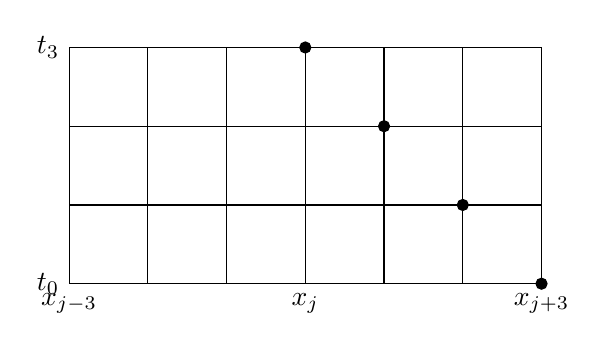
\begin{tikzpicture}
        \draw (0,0) node[below] {$x_{j-3}$} node[left] {$t_0$};
        \draw (0,0)--(0,3);
        \draw (1,0)--(1,3);
        \draw (2,0)--(2,3);
        \draw (3,0)--(3,3);
        \draw (3,0) node[below] {$x_j$};
        \draw (4,0)--(4,3);
        \draw (5,0)--(5,3);
        \draw (6,0)--(6,3);
        \draw (6,0) node[below] {$x_{j+3}$};
        \draw (0,0)--(6,0);
        \draw (0,1)--(6,1);
        \draw (0,2)--(6,2);
        \draw (0,3)--(6,3);
        \draw (0,3) node[left] {$t_3$};
        \filldraw [black] (6,0) circle (2pt);
        \filldraw [black] (5,1) circle (2pt);
        \filldraw [black] (4,2) circle (2pt);
        \filldraw [black] (3,3) circle (2pt);
      \end{tikzpicture}
      \centerline{$\mu=-1$}
    \end{minipage}
  \end{figure}
\end{solution}

\begin{prob}[Exercise 11.92]
  Show that the modified equation of the leapfrog method is also (11.96).
  However, if one more term of higher-order derivative had been retained,
  the modified equation of the leapfrog method would have been
  \begin{equation*}
    v_t + av_x + \dfrac{ah^2}6(1-\mu^2)v_{xxx} = \epsilon_fv_{xxxxx}
  \end{equation*}
  while that of the Lax-Wendroff method would have been
  \begin{equation*}
    v_t + av_x + \dfrac{ah^2}6(1-\mu^2)v_{xxx} = \epsilon_wv_{xxxx}.
  \end{equation*}
\end{prob}

\begin{solution}
  先考虑 leapfrog 方法
  \begin{equation*}
    \dfrac{U_j^{n+1} - U_j^{n-1}}{2k} = -\dfrac{a}{2h}(U_{j+1}^n - U_{j-1}^n).
  \end{equation*}
  将 $U_j^n$ 替换为 $v(x,t)$ 得
  \begin{equation*}
    \dfrac{v(x,t+k) - v(x,t-k)}{2k} = -\dfrac{a}{2h}(v(x+h,t) - v(x-h,t)).
  \end{equation*}
  在 $(x,t)$ 处泰勒展开至五阶,得
  \begin{equation*}
    v_t + \dfrac{k^2}6v_{ttt} + \dfrac{k^4}{120}v_{ttttt} = -a\left(v_x + \dfrac{h^2}6v_{xxx} + \dfrac{h^4}{120}v_{xxxxx}\right).
  \end{equation*}
  即(假设 $k=O(h)$)
  \begin{equation*}
    v_t + av_x = -\dfrac 16(k^2v_{ttt} + ah^2v_{xxx}) - \dfrac 1{120}(k^4v_{ttttt} + ah^4v_{xxxxx}) + O(h^6).
  \end{equation*}
  因为
  \begin{equation*}
    \begin{aligned}
      v_{ttttt} = & -a^5v_{xxxxx} + O(h^2), & \\
      v_{ttt} = & -av_{xtt} - \dfrac 16(k^2v_{ttttt} + ah^2v_{xxxtt}) + O(h^4) & \\
      = & a^2v_{xxt} + \dfrac a6(k^2v_{xtttt} + ah^2v_{xxxxt}) - \dfrac 16(k^2a^5v_{xxxxx} + h^2a^3v_{xxxxx}) + O(h^4) & \\
      = & -a^3v_{xxx} - \dfrac {a^2}6(k^2v_{xxttt} + ah^2v_{xxxxx}) + \dfrac a6(k^2a^4v_{xxxxx} - h^2a^2v_{xxxxx}) - \dfrac 16(k^2a^5-h^2a^3)v_{xxxxx} + O(h^4) & \\
      = & -a^3v_{xxx} + \dfrac 12(k^2a^5 - h^2a^3)v_{xxxxx} + O(h^4), & \\
    \end{aligned}
  \end{equation*}
  所以
  \begin{equation*}
    v_t + av_x + \dfrac{k^2}6\left(-a^3v_{xxx} + \dfrac 12(k^2a^5-h^2a^3)v_{xxxxx}\right) - \dfrac{k^4}{120}a^5v_{xxxxx} + \dfrac{ah^2}6v_{xxx} + \dfrac{ah^4}{120}v_{xxxxx} + O(h^6) = 0.
  \end{equation*}
  代入 $\mu = \dfrac{ak}{h}$ 整理得
  \begin{equation*}
    v_t + av_x + \dfrac{ah^2}6(1-\mu^2)v_{xxx} + \dfrac{ah^4}{120}(1-10\mu^2+9\mu^4)v_{xxxxx} + O(h^6) = 0.
  \end{equation*}
  因此,保留到三阶的方程为
  \begin{equation*}
    v_t + av_x + \dfrac{ah^2}6(1-\mu^2)v_{xxx} = 0,
  \end{equation*}
  保留到五阶的方程为
  \begin{equation*}
    v_t + av_x + \dfrac{ah^2}6(1-\mu^2)v_{xxx} + \dfrac{ah^4}{120}(1-10\mu^2+9\mu^4)v_{xxxxx} = 0.
  \end{equation*}
  再考虑 Lax-Wendroff 方法
  \begin{equation*}
    U_j^{n+1} - U_j^n = -\dfrac{\mu}2(U_{j+1}^n - U_{j-1}^n) + \dfrac{\mu^2}2(U_{j+1}^n - 2U_j^n + U_{j-1}^n).
  \end{equation*}
  将 $U_j^n$ 替换为 $v(x,t)$ 得
  \begin{equation*}
    v(x,t+k) - v(x,t) = -\dfrac{\mu}2(v(x+h,t)-v(x-h,t)) + \dfrac{\mu^2}2(v(x+h,t)-2v(x,t)+v(x-h,t)).
  \end{equation*}
  在 $(x,t)$ 处泰勒展开至四阶,得
  \begin{equation*}
    kv_t+\dfrac{k^2}2v_{tt}+\dfrac{k^3}6v_{ttt}+\dfrac{k^4}{24}v_{tttt}+O(h^5)
    =-\mu\left(hv_x+\dfrac{h^3}6v_{xxx}+O(h^5)\right) + \mu^3(\dfrac{h^2}2v_{xx}+\dfrac{h^4}{24}v_{xxxx}+O(h^6)).
  \end{equation*}
  因为
  \begin{equation*}
    \begin{aligned}
      v_{tttt} = & a^4v_{xxxx} + O(h), & \\
      v_{ttt} = & -av_{xtt} - \dfrac k2v_{tttt} + \dfrac{\mu ah}2v_{xxtt} + O(h^2) & \\
      = & -a\left(-av_{xxt} - \dfrac k2v_{xttt} + \dfrac{\mu ah}2v_{xxxt}\right) - \dfrac k2 a^4v_{xxxx} + \dfrac{\mu a^3h}2v_{xxxx} + O(h^2) & \\
      = & a^2\left(-av_{xxx} - \dfrac k2v_{xxtt} + \dfrac{\mu ah}2v_{xxxx}\right) - \dfrac k2 a^4v_{xxxx} + \dfrac{\mu a^3h}2v_{xxxx} + O(h^2) & \\
      = & -a^3v_{xxx} + O(h^2), & \\
      v_{tt} = & -av_{xt} - \dfrac k2v_{ttt} + \dfrac{\mu ah}2v_{xxt} - \dfrac{k^2}6 v_{tttt} - \dfrac{ah^2}6v_{xxxt} + O(h^3) & \\
      = & -a\left(-av_{xx} - \dfrac k2v_{xtt} + \dfrac{\mu ah}2v_{xxx} - \dfrac{k^2}6 v_{xttt} - \dfrac{ah^2}6v_{xxxx}\right) + \dfrac{ka^3}2v_{xxx} - \dfrac{\mu a^2h}2v_{xxx} - \dfrac{k^2a^4}6 v_{xxxx} - \dfrac{a^2h^2}6v_{xxxx} + O(h^3) & \\
      = & a^2v_{xx} + \dfrac{a^2h^2}3(1-\mu^2)v_{xxxx} + O(h^3), & \\
    \end{aligned}
  \end{equation*}
  代入泰勒展开式,整理得
  \begin{equation*}
    v_t + av_x + \dfrac{ah^2}6(1-\mu^2)v_{xxx} + \dfrac{ah^3}8(\mu-\mu^3)v_{xxxx} + O(h^4) = 0.  
  \end{equation*}
  因此保留到四阶的方程为
  \begin{equation*}
    v_t + av_x + \dfrac{ah^2}6(1-\mu^2)v_{xxx} + \dfrac{ah^3}8(\mu-\mu^3)v_{xxxx} = 0.
  \end{equation*}
\end{solution}

\begin{prob}[Exercise 11.93]
  Show that the modified equation of the Beam-Warming method aplied to the advection equation (11.56) with $a\geq 0$ is
  \begin{equation*}
    v_t + av_x + \dfrac{ah^2}6(-2+3\mu-\mu^2)v_{xxx} = 0.
  \end{equation*}
  Thus we have
  \begin{equation*}
    \begin{aligned}
      C_p(\xi) = a + \dfrac{ah^2}6(\mu-1)(\mu-2)\xi^2,\\
      C_g(\xi) = a + \dfrac{ah^2}2(\mu-1)(\mu-2)\xi^2.\\      
    \end{aligned}
  \end{equation*}
  How do these facts answer Question (e) of Example 11.87?
\end{prob}

\begin{solution}
  Beam-Warming 方法的半离散格式
  \begin{equation*}
    U_j^{n+1} = U_j^n - \dfrac {\mu}2(3U_j^n - 4U_{j-1}^n + U_{j-2}^n) + \dfrac {\mu^2}2(U_j^n - 2U_{j-1}^n + U_{j-2}^n)
  \end{equation*}
  中 $U_j^n$ 替换为 $v(x,t)$ 得
  \begin{equation*}
    v(x,t+k) - v(x,t) = -\dfrac {\mu}2(3v(x,t) - 4v(x-h,t) + v(x-2h,t)) + \dfrac {\mu^2}2(v(x,t) - 2v(x-h,t) + v(x-2h,t)).
  \end{equation*}
  在 $(x,t)$ 处泰勒展开至三阶,得
  \begin{equation*}
    kv_t + \dfrac{k^2}2v_{tt} + \dfrac{k^3}6v_{ttttt} + O(k^4) = -\dfrac {\mu}2\left(hv_x - \dfrac 23v_{xxx}\right) + \dfrac{\mu^2}2(h^2v_{xx} - h^3v_{xxx}).
  \end{equation*}
  因为
  \begin{equation*}
    v_{ttt} = -a^3v_{xxx} + O(h),
  \end{equation*}
  \begin{equation*}
    \begin{aligned}
      v_{tt} = & -av_{xt} - \dfrac k2v_{ttt} + \dfrac{\mu ah}2v_{xxt} + O(h^2) & \\
      = & -a\left(-av_{xx} - \dfrac k2v_{xtt} + \dfrac{\mu ah}2v_{xxx}\right) + \dfrac k2a^3v_{xxx} - \dfrac{\mu a^2h}v_{xxx} + O(h^2) & \\
      = & a^2v_{xx} + O(h^2),
    \end{aligned}
  \end{equation*}
  代入泰勒展开式得
  \begin{equation*}
    v_t + av_x + \dfrac 16ah^2(-2+3\mu-\mu^2)v_{xxx}+O(h^3) = 0.
  \end{equation*}
  故保留到三阶的方程为
  \begin{equation*}
    v_t + av_x + \dfrac 16ah^2(-2+3\mu-\mu^2)v_{xxx} = 0.
  \end{equation*}
  因此
  \begin{equation*}
    \begin{aligned}
      \omega(\xi) = & a\xi + \dfrac{ah^2}6(2-3\mu+\mu^2)\xi^3 = a\xi + \dfrac{ah^2}6(\mu-1)(\mu-2)\xi^3, \\
      C_p(\xi) = & \dfrac{\omega(\xi)}{\xi} = a + \dfrac{ah^2}6(\mu-1)(\mu-2)\xi^2, \\
      C_g(\xi) = & \dfrac{\dd\omega(\xi)}{\dd\xi} = a + \dfrac{ah^2}2(\mu-1)(\mu-2)\xi^2. \\
    \end{aligned}
  \end{equation*}
  当 $0<\mu<1$ 时,$|C_p(\xi)|>|a|$。在 Example 11.87 中,$\mu = 0.8$,
  因此 Beam-Warming 方法求出的解的峰值更高,且峰值出现的时间比真解要早。
\end{solution}

\begin{prob}[Exercise 11.94]
  What if $\mu=1$? Discuss this case for both Lax-Wendroff and leapfrog methods
  to answer Question (f) of Example 11.87.
\end{prob}

\begin{solution}
  当 $\mu=1$ 时,Lax-Wendroff 方法的半离散格式退化为 $U_j^{n+1} = U_{j-1}^n$。
  此时,显然所有格点处的解均为精确的:$U_j^n = U_{j-n}^0 = \eta(jh-nak) = \eta((j-n)h)$。
  leapfrog 方法的半离散格式退化为 $U_j^{n+1} = U_j^{n-1} - U_{j+1}^n + U_{j-1}^n$。
  我们归纳证明所有格点处的解均为精确的。
  $U_j^0 = \eta(jh)$ 的值由初值条件直接给出,是精确的;假设 $U_j^n$ 为精确的,即 $U_j^n = \eta((j-n)h)$,
  则 $U_j^{n+1} = U_j^{n-1} - U_{j+1}^n + U_{j-1}^n = \eta((j-n+1)h) - \eta((j+1-n)h) + \eta((j-1-n)h) = \eta((j-1-n)h)$
  是精确解。故归纳成立。
  综上,$\mu=1$ 时 Lax-Wendroff 和 leapfrog 方法都可以得到精确解。
\end{solution}

\begin{prob}[Exercise 11.96]
  Apply the von Neumann analysis to the Lax-Friedrichs method to derive its amplification factor as
  \begin{equation*}
    g(\xi h) = \cos(\xi h) - \mu\ii\sin(\xi h).
  \end{equation*}
  For which values of $\mu$ would the method be stable?
\end{prob}

\begin{solution}
  Lax-Friedrichs 方法的半离散格式为
  \begin{equation*}
    U_j^{n+1} = \dfrac 12(U_{j+1}^n + U_{j-1}^n) - \dfrac{\mu}2(U_{j+1}^n - U_{j-1}^n).
  \end{equation*}
  两端同时作 Fourier 变换得
  \begin{equation*}
    \dfrac 1{\sqrt{2\pi}}\int_{-\frac{\pi}h}^{\frac{\pi}h}e^{\ii jh\xi}\hat{U}^{n+1}(\xi)\dd\xi
    = \dfrac 1{\sqrt{2\pi}}\int_{-\frac{\pi}h}^{\frac{\pi}h}\left[\dfrac 12(e^{\ii(j+1)h\xi} + e^{\ii(j-1)h\xi}) - \dfrac{\mu}2(e^{\ii(j+1)h\xi} - e^{\ii(j-1)h\xi})\right]\hat{U}^n(\xi)\dd\xi.
  \end{equation*}
  右端可化简为
  \begin{equation*}
    \dfrac 1{\sqrt{2\pi}}\int_{-\frac{\pi}h}^{\frac{\pi}h}e^{\ii jh\xi}(\cos h\xi - \mu\ii\sin h\xi)\hat{U}^n(\xi)\dd\xi.
  \end{equation*}
  因此 $g(\xi) = \cos h\xi - \mu\ii\sin h\xi$。
  由 $|g(\xi)|\leq 1$ 得
  \begin{equation*}
    \cos^2 h\xi + \mu^2\sin^2 h\xi \leq 1
  \end{equation*}
  即
  \begin{equation*}
    1 + (\mu^2-1)\sin^2 h\xi \leq 1.
  \end{equation*}
  因为 $0\leq \sin^2 h\xi \leq 1$,所以要使上式对任意 $\xi$ 成立,需要 $|\mu|\leq 1$。
  即 $|\mu|\leq 1$ 时方法稳定。
\end{solution}

\begin{prob}[Exercise 11.97]
  Apply the von Neumann analysis to the Lax-Wendroff method to derive its amplification factor as
  \begin{equation*}
    g(\xi h) = 1-2\mu^2\sin^2\dfrac{\xi h}2 - \ii\mu\sin(\xi h).
  \end{equation*}
  For which values of $\mu$ would the method be stable?
\end{prob}

\begin{solution}
  Lax-Wendroff 方法的半离散格式为
  \begin{equation*}
    U_j^{n+1} = U_j^n - \dfrac{\mu}2(U_{j+1}^n - U_{j-1}^n) + \dfrac{\mu^2}2(U_{j+1}^n - 2U_j^n + U_{j-1}^n).
  \end{equation*}
  两端同时作 Fourier 变换得
  \begin{equation*}
    \dfrac 1{\sqrt{2\pi}}\int_{-\frac{\pi}h}^{\frac{\pi}h}e^{\ii jh\xi}\hat{U}^{n+1}(\xi)\dd\xi
    = \dfrac 1{\sqrt{2\pi}}\int_{-\frac{\pi}h}^{\frac {\pi}h}e^{\ii jh\xi}\left(1-\mu\ii\sin h\xi-2\mu^2\sin^2\dfrac{h\xi}2\right)\hat{U}^n(\xi)\dd\xi.
  \end{equation*}
  因此
  \begin{equation*}
    g(\xi) = 1-\mu\ii\sin h\xi-2\mu^2\sin^2\dfrac{h\xi}2.    
  \end{equation*}
  由 $|g(\xi)|\leq 1$ 得
  \begin{equation*}
    (1-2\mu^2\sin^2\dfrac{h\xi}2)^2 + \mu^2\sin^2 h\xi \leq 1,
  \end{equation*}
  即
  \begin{equation*}
    (1-\mu^2(1-\cos h\xi))^2 + \mu^2\sin^2 h\xi \leq 1,
  \end{equation*}
  即
  \begin{equation*}
    (\mu^4-\mu^2)(1-\cos h\xi)^2\leq 0.
  \end{equation*}
  故 $|\mu|\leq 1$。即 $|\mu|\leq 1$ 时方法稳定。
\end{solution}

\nocite{*}
\printbibliography[heading=bibintoc, title=\ebibname]

\end{document}